



\documentclass{beamer}
\usepackage{multimedia}
\usepackage{graphicx}
\usetheme{Madrid}

\usepackage{amsmath,amssymb}
\usepackage{bm}
\usepackage[absolute,overlay]{textpos}
\usepackage{mathtools}
\usepackage{courier}
\usepackage{tikz}
\usepackage{caption}
\usepackage{lmodern}
\beamertemplatenavigationsymbolsempty
\usefonttheme[onlymath]{serif}
\graphicspath{{./gfx/}}

\newcommand{\ppos}{q}
\newcommand{\pvel}{u}
\newcommand{\fpos}{r}
\newcommand{\fvel}{v}
\newcommand{\corr}{\text{corr}}
\newcommand{\dpr}{\text{\tiny DP}}
\newcommand{\qtd}{\text{\tiny q2D}}
\renewcommand{\vec}[1]{\bm{#1}}
\newcommand{\tens}[1]{\bm{\mathcal{#1}}}
\newcommand{\oper}[1]{\mathcal{#1}}
\newcommand{\uammd}{\gls{UAMMD}\xspace}
\newcommand{\gpu}{\gls{GPU}\xspace}
\newcommand{\dt}{\delta t}
\newcommand{\kT}{k_B T}
\newcommand{\sinc}{\textrm{sinc}}
\newcommand{\floor}{\textrm{floor}}
\newcommand{\near}{\textrm{near}}
\newcommand{\far}{\textrm{far}}
\newcommand{\half}{\frac{1}{2}}
\newcommand{\red}[1]{{\color{red}#1}}
\newcommand{\fou}[1]{\widehat{#1}}
\newcommand{\noise}{\widetilde{W}}

\newcommand{\executeiffilenewer}[3]{
  \ifnum
  \pdfstrcmp{\pdffilemoddate{#1}}{\pdffilemoddate{#2}}>0
  {\immediate\write18{#3}}
  \fi
}
\newcommand{\includesvg}[2][width=\columnwidth]{
  \executeiffilenewer{#2.svg}{#2.pdf}
  {inkscape -D #2.svg --export-type=pdf } %  --export-latex}
  %\def\svgwidth{#2}
  % \input{#1.pdf_tex}
  \includegraphics[#1]{#2.pdf}
}

\usepackage[absolute,overlay]{textpos}

\def\ucpp{uammd_cpp_lexer.py:UAMMDCppLexer -x}
\usepackage{tcolorbox}
\usepackage{xparse}
\tcbuselibrary{breakable,minted,xparse,skins,listings}
\usemintedstyle{default}
\setminted[\ucpp]{ %
  linenos=false,             % Line numbers
  autogobble=true,          % Automatically remove common white space
  fontsize=\small,
  breaklines
}
\AtBeginDocument{
  \newtcblisting{code2}[2][]{
    colback=white,
    colbacktitle=white,
    coltitle=black,
    pad at break*=0mm,
    listing only,
    listing engine=minted,
    listing remove caption=true,
    title={~#1},
    minted language=\ucpp,
    enhanced jigsaw,
    minipage boxed title,
    attach boxed title to bottom center={xshift=0mm,yshift=-1mm},
    boxed title style={size=small, blanker},
    center title,
    #2
  }
}
\tcbsetforeverylayer{autoparskip}

\title{Complex fluids in the GPU era}
\subtitle{Algorithms and simulations}
\author{Raul P. Pelaez}

\institute{Universidad Autónoma de Madrid}
\date{\today}

%\captionsetup[figure]{font=small,skip=0pt}
\usepackage[export]{adjustbox}
\begin{document}


\begin{frame}
  \titlepage
\end{frame}

\begin{frame}
  \tableofcontents
\end{frame}




\section{Contents}
\begin{frame}
  \frametitle{\insertsection}
  \begin{itemize}
  \item UAMMD's functionalities
  \item Particle-based and grid based
  \item Code structure
    \begin{itemize}
    \item open-source
    \item adaptable
    \item ...
    \end{itemize}
  \end{itemize}
\end{frame}
\section{Contributions}
\begin{frame}
  \frametitle{This thesis Contributions}
  \begin{itemize}
  \item A list of contributions: UAMMD, new algorithms, new physics.
  \item Use this slide to give an outline of the talk
  \end{itemize}
\end{frame}
\section{Introduction}
\subsection{UAMMD: Universally Adaptable Multiscale Molecular Dynamics}
\begin{frame}[t]
  \frametitle{Introduction}
  \framesubtitle{UAMMD: Universally Adaptable Multiscale Molecular Dynamics}
  \begin{overprint}
    \onslide<+>
    \centering \huge \bf Universal
    \onslide<+>
    \centering \huge \bf Adaptable
    \onslide<+>
    \centering \huge \bf Multiscale
    \onslide<+>
    \centering \huge \bf Molecular Dynamics
  \end{overprint}
  \begin{columns}[T]
    \begin{column}{0.65\linewidth}
      \begin{overlayarea}{\linewidth}{0.6\paperheight}
        \begin{figure}
          \only<1>{%
            \includesvg[width=0.9\linewidth]{gfx/universally}%
          }%
          \only<2>{%
            \includesvg[width=0.8\linewidth]{gfx/virus}%
          }%
          \only<3>{%
            \includesvg[width=0.8\linewidth]{gfx/scales}%
          }%
          \only<4>{%
            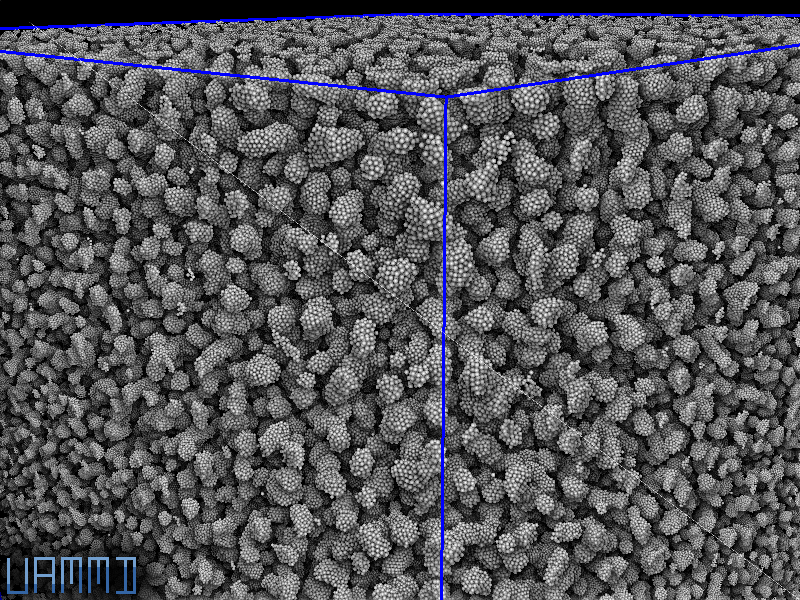
\includegraphics[width=0.9\linewidth]{shotlogo}%
          }%
        \end{figure}
      \end{overlayarea}
    \end{column}
    \begin{column}{0.35\linewidth}      
      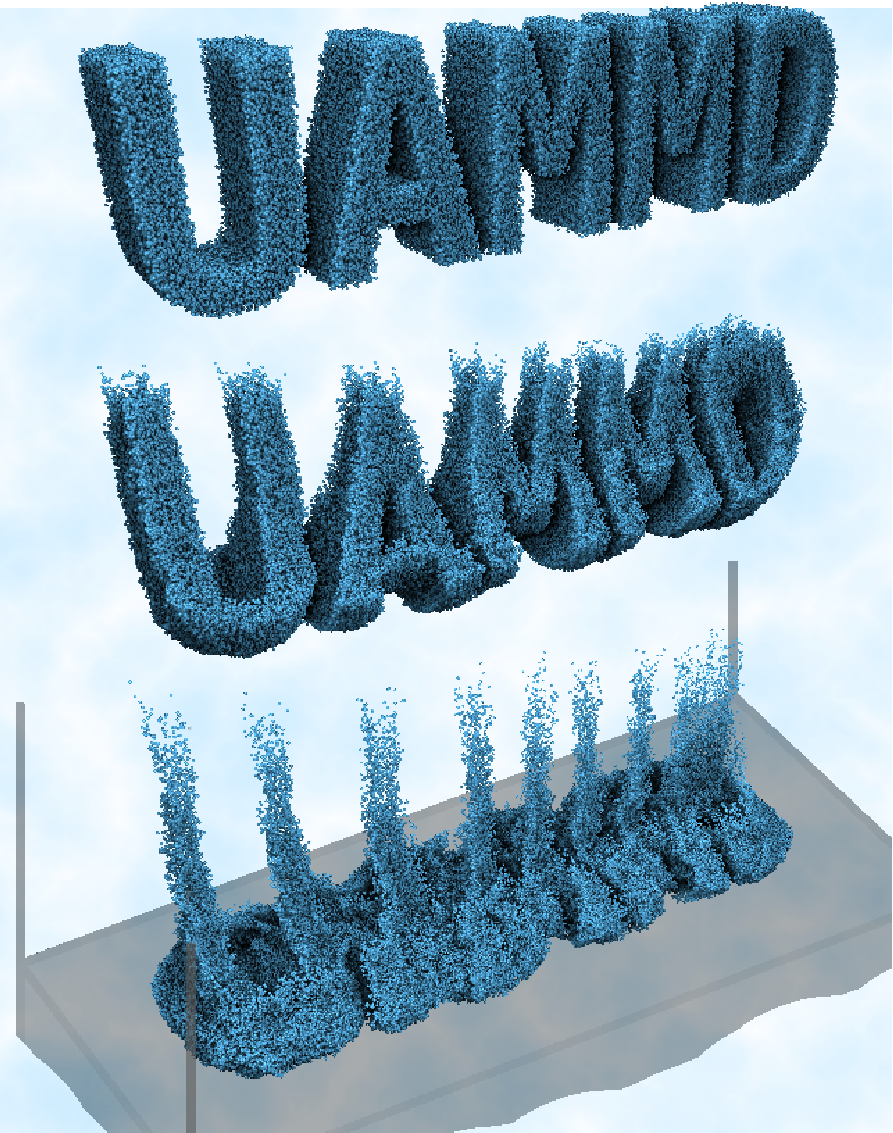
\includegraphics[width=1.0\linewidth]{poster.png}
     \end{column}
   \end{columns}
   \only<1>{\Large Lagrangian and Eulerian descriptions.}%
   \only<2>{\Large Independent building blocks.}%
   \only<3>{\Large Solvers for many scales.}%
   \only<4>{\Large Mainly particle based.}%
\end{frame}


\subsection{Complex fluids}
\begin{frame}
  \frametitle{Complex fluids}
  \framesubtitle{The spatio-temporal landscape of numerical techniques.}
  \begin{figure}
    \centering
    \includesvg[width=0.8\linewidth]{gfx/landscape}
    \caption{Figure courtesy of Rafael Delgado-Buscalioni.}
  \end{figure}
\end{frame}

\begin{frame}
  \frametitle{Complex fluids}
  \framesubtitle{Usual levels of coarse-grained description}
  \begin{figure}
    \centering
    \includesvg[width=0.55\linewidth]{gfx/multiscale}
  \end{figure}  
\end{frame}
\begin{frame}[t]
  \frametitle{Complex fluids}
  \framesubtitle{Usual levels of coarse-grained description}
  \begin{columns}[T]
    \begin{column}{0.5\linewidth}
        \begin{tikzpicture}
          \node[anchor = south west, inner sep = 0] (image) {\includesvg[width=\linewidth]{gfx/multiscale}};
          \begin{scope}[shift={(image.south west)},x={(image.south east)},y={(image.north west)}]
            %Draw a overlaying grid to easily see where the rectangles must be, this can be commented out in the final version
%            \draw foreach \xy in {0,0.1,...,1.001}{
%            (\xy,0) -- node[pos=0,below]{\pgfmathprintnumber{\xy}} (\xy,1)
%            (0,\xy) -- node[pos=0,left]{\pgfmathprintnumber{\xy}} (1,\xy)};
            \foreach[count=\i] \mypath in {
              {(0,1) rectangle (0.48,0.55)},
              {(0,0.55) rectangle (0.48,0)},
              {(0.48,1) rectangle (1.0,0.55)},
              {(0.48,0.55) rectangle (1,0)},
              {(0,1) rectangle (1,0)},
              {(0,1) rectangle (1,0)}
            }{
              \filldraw<\i>[white,opacity=0.9,even odd rule] (0,0) rectangle (1,1) \mypath;
            }
          \end{scope}
        \end{tikzpicture}
      \end{column}
      \begin{column}{0.45\linewidth}
      \begin{center}
        \textbf{Relevant variables:}
      \end{center}
      \begin{itemize}
      \item<1-> $\vec{q}_i$: Position of particle $i$.
      \item<1-3,5-> $\vec{u}_i$: Velocity of particle $i$.
      \item<2,5-> $\xi(\vec{q}_{ij})$: Friction kernel.
      \item<3,5-> $\vec{v}(\vec{r},t)$: Fluid velocity field.
      \item<4-> $M(\vec{q}_{ij})$: Mobility tensor.
      \end{itemize}
      \centering      
      \only<1-4>{\textbf{Tipical timescale:}\newline}
      \only<1>{$\tau \sim 10^{-12}s$}
      \only<2>{$\tau \sim 10^{-5}s$}
      \only<3>{$\tau \sim 10^{-\{9-6\}}s$}
      \only<4>{$\tau \sim 10^{-3}s$}
      \only<5->{\textbf{Timescale range:}\newline $\tau \sim [10^{-12}, 10^{-3}]s$}
    \end{column}
  \end{columns}
  \only<1>{\begin{textblock*}{0.5\linewidth}(0.05\linewidth, 0.55\paperheight)}
  \only<2>{\begin{textblock*}{0.5\linewidth}(0.05\linewidth, 0.2\paperheight)}
  \only<3>{\begin{textblock*}{0.53\linewidth}(0.05\linewidth, 0.49\paperheight)}
  \only<4,5>{\begin{textblock*}{0.5\linewidth}(0.05\linewidth, 0.17\paperheight)}
  \only<6>{\begin{textblock*}{0.99\linewidth}(0.04\linewidth,0.23\paperheight)}
    \begin{block}<1-4>{
        \only<1>{Molecular Dynamics (MD)}
        \only<2>{Langevin Dynamics (LD)}
        \only<3>{Immersed Boundary Method (IBM)}
        \only<4>{Brownian Dynamics (BD)}
      }{$$\only<1>{%
          \begin{aligned}
            m\ddot{\vec{\ppos}} &= \vec{F}\\
            \vec{\pvel} &= \dot{\vec{\ppos}}
          \end{aligned}
        }%
        \only<2>{m d\vec{\pvel} = \vec{F}dt - \xi\vec{\pvel}dt +  \sqrt{2\xi\kT}\vec{\noise}}%
        \only<3>{%
          \begin{aligned}
            &\rho\partial_t\vec{\fvel} = -\vec{\partial}_{\vec{\fpos}}\cdot \tens{\sigma} + \vec{f} + \text{fluct}\\
            \int_{V_p}\vec{f}d\vec{\fpos} &= \vec{F}\quad\text{and}\quad \vec{u} = \int_{V_p}\vec{\fvel}(\vec{\fpos}, t)d\vec{\fpos}
          \end{aligned}%
        }%
      \only<4>{%
          \begin{aligned}%
            d\vec{\ppos} =& \tens{M}\vec{F}dt + \sqrt{2\kT\tens{M}}d\vec{\noise}\\%
                          &+ \kT\vec{\partial}_{\vec{\ppos}}\cdot\tens{M}dt.%
          \end{aligned}%
        }%
        $$}
    \end{block}
    \begin{alertblock}<6>{\centering \Large We always have}
      \centering \Large
      Interacting ``particles'' with a state that ``evolves'' in time.
    \end{alertblock}
  \end{textblock*}

  \only<1>{
    \centering
    Supervector notation $\vec{q} := \{\vec{q}_1,\dots,\vec{q}_N\}$
  }
  \only<2>{
    \centering
    $\vec{\noise}$: Wienner increments, $\mathcal{N}(0,dt)$
  }
  \only<3>{
    \centering
    $\partial_t := \frac{\partial}{\partial t} \rightarrow \vec{\partial}_{\vec{r}} := \nabla := \left(\partial_x,\partial_y,\partial_z\right) $ 
  }
  \only<4>{
    \centering
    $d\vec{\noise}$: Wienner increments, $\mathcal{N}(0,dt)$
  }
\end{frame}

\section{UAMMD's functionalities}
\begin{frame}[fragile]
  \frametitle{UAMMD}
  \framesubtitle{Conceptual hierarchy}
  \includesvg[width=\linewidth]{gfx/sketchUAMMD}
  \begin{overprint}
    \onslide<2>
    \begin{code2}[]{label=code:module}
      #include<uammd.cuh>
      int main(int argc, char* argv[]){
        auto sys = std::make_shared<System>(argc, argv);
        ...
    \end{code2}
    \onslide<3>
    \begin{code2}[]{label=code:module}
      #include<uammd.cuh>
      int main(int argc, char* argv[]){
        auto sys = std::make_shared<System>(argc, argv);
        const int nP = 1e6; //Number of particles
        auto pd = std::make_shared<ParticleData>(nP, sys);
        ...
      \end{code2}
      \onslide<4>
    \begin{code2}[]{label=code:module}
      ...
      auto pos = pd->getPos(access::cpu, access::write);
      pos[0] = {1,1,1,0}; // x,y,x, color (type)
      ...
    \end{code2}
    \onslide<5>
    \begin{code2}[]{label=code:module}
      ...
      auto md = std::make_shared<VerletNVE>(pd, /*Parameters*/);
      md->forwardTime(); //Exposed by every Integrator
      ...      
    \end{code2}
    \onslide<6>
    \begin{code2}[]{label=code:module}
      ...
      auto electro = std::make_shared<Poisson>(pd,
                                              /*Parameters*/);
      //Exposed by every Integrator
      md->addInteractor(electro); 
      md->forwardTime();
      ...      
    \end{code2}
  \end{overprint}
\end{frame}

\section{Introduction}
\begin{frame}
  \frametitle{\insertsection}
  \begin{itemize}
  \item Outline
  \item Physics, algorithms and implementation
  \item This thesis contributions
  \end{itemize}
\end{frame}

\subsection{Complex fluids}
\begin{frame}
  \frametitle{\insertsubsectionnavigation{\linewidth}}
  \begin{itemize}
  \item What a complex fluid is and why we care
  \item Coarse-graining
  \end{itemize}
\end{frame}
\subsubsection{A typical system of interest}
\begin{frame}
  \frametitle{\insertsubsectionnavigation{\linewidth}} 
  \framesubtitle{\insertsubsubsection}
  \begin{itemize}
  \item ``We want to study this particular system (a virus?, QCM?)''
  \item Problems that arise when trying to simulate this system
  \item The message is: We need new theory and algorithms. If we carefully design a software for a system like this, we end up with something that is also valid for things like MD,  SPH, DPD,...
  \end{itemize}
\end{frame}
\subsection{High performance computing in complex fluids}
\begin{frame}
  \frametitle{\insertsubsectionnavigation{\linewidth}} 
  \begin{itemize}
  \item The GPU
  \item Other software packages
  \item Trying to keep it simple
  \end{itemize}
\end{frame}


\section{The different ingredients of a complex fluid simulation}

\begin{frame}
  \frametitle{\insertsectionnavigation{\linewidth}} 
  \begin{itemize}
  \item Hydrodynamics
  \item Particle interactions
  \item Electrostatics
  \end{itemize}
\end{frame}

\subsection{Hydrodynamics}
\begin{frame}
  \frametitle{\insertsubsectionnavigation{\linewidth}}
  \begin{itemize}
  \item Fluid dynamics
  \item Particle-fluid coupling (IBM)
  \item Pseudo-spectral solvers (FCM)
  \end{itemize}
\end{frame}

\subsection{Particle interactions}
\begin{frame}
  \frametitle{\insertsubsectionnavigation{\linewidth}}
  \begin{itemize}
  \item Neighbour lists
  \item bonds
  \end{itemize}
\end{frame}

\subsection{Electrostatics}
\begin{frame}
  \frametitle{\insertsubsectionnavigation{\linewidth}}
  \begin{itemize}
  \item Poisson equation
  \item Reuse of FCM
  \end{itemize}  
\end{frame}
    
\subsection{UAMMD: A GPU framework for complex fluids}
\begin{frame}
  \frametitle{\insertsubsectionnavigation{\linewidth}} 
  \begin{itemize}
  \item What UAMMD is and tries to achieve
  \item ``UAMMD has enabled the community to study hydrodynamics in new systems''
  \item Not trying to sell UAMMD, just showcase what it can do.    
  \end{itemize}
\end{frame}

\section{New physics}

\begin{frame}
  \frametitle{\insertsectionnavigation{\linewidth}} 
  \begin{itemize}
  \item List works using UAMMD, what level of detail here?
  \end{itemize}
\end{frame}

\end{document}